\documentclass[journal,12pt,twocolumn]{IEEEtran}

\usepackage{setspace}
\usepackage{gensymb}

\singlespacing


\usepackage[cmex10]{amsmath}

\usepackage{amsthm}

\usepackage{mathrsfs}
\usepackage{txfonts}
\usepackage{stfloats}
\usepackage{bm}
\usepackage{cite}
\usepackage{cases}
\usepackage{subfig}

\usepackage{longtable}
\usepackage{multirow}

\usepackage{enumitem}
\usepackage{mathtools}
\usepackage{steinmetz}
\usepackage{tikz}
\usepackage{circuitikz}
\usepackage{verbatim}
\usepackage{tfrupee}
\usepackage[breaklinks=true]{hyperref}
\usepackage{graphicx}
\usepackage{tkz-euclide}

\usetikzlibrary{calc,math}
\usepackage{listings}
    \usepackage{color}                                            %%
    \usepackage{array}                                            %%
    \usepackage{longtable}                                        %%
    \usepackage{calc}                                             %%
    \usepackage{multirow}                                         %%
    \usepackage{hhline}                                           %%
    \usepackage{ifthen}                                           %%
    \usepackage{lscape}     
\usepackage{multicol}
\usepackage{chngcntr}

\DeclareMathOperator*{\Res}{Res}

\renewcommand\thesection{\arabic{section}}
\renewcommand\thesubsection{\thesection.\arabic{subsection}}
\renewcommand\thesubsubsection{\thesubsection.\arabic{subsubsection}}

\renewcommand\thesectiondis{\arabic{section}}
\renewcommand\thesubsectiondis{\thesectiondis.\arabic{subsection}}
\renewcommand\thesubsubsectiondis{\thesubsectiondis.\arabic{subsubsection}}


\hyphenation{op-tical net-works semi-conduc-tor}
\def\inputGnumericTable{}                                 %%

\lstset{
%language=C,
frame=single, 
breaklines=true,
columns=fullflexible
}
\begin{document}


\newtheorem{theorem}{Theorem}[section]
\newtheorem{problem}{Problem}
\newtheorem{proposition}{Proposition}[section]
\newtheorem{lemma}{Lemma}[section]
\newtheorem{corollary}[theorem]{Corollary}
\newtheorem{example}{Example}[section]
\newtheorem{definition}[problem]{Definition}

\newcommand{\BEQA}{\begin{eqnarray}}
\newcommand{\EEQA}{\end{eqnarray}}
\newcommand{\define}{\stackrel{\triangle}{=}}
\bibliographystyle{IEEEtran}
\providecommand{\mbf}{\mathbf}
\providecommand{\pr}[1]{\ensuremath{\Pr\left(#1\right)}}
\providecommand{\qfunc}[1]{\ensuremath{Q\left(#1\right)}}
\providecommand{\sbrak}[1]{\ensuremath{{}\left[#1\right]}}
\providecommand{\lsbrak}[1]{\ensuremath{{}\left[#1\right.}}
\providecommand{\rsbrak}[1]{\ensuremath{{}\left.#1\right]}}
\providecommand{\brak}[1]{\ensuremath{\left(#1\right)}}
\providecommand{\lbrak}[1]{\ensuremath{\left(#1\right.}}
\providecommand{\rbrak}[1]{\ensuremath{\left.#1\right)}}
\providecommand{\cbrak}[1]{\ensuremath{\left\{#1\right\}}}
\providecommand{\lcbrak}[1]{\ensuremath{\left\{#1\right.}}
\providecommand{\rcbrak}[1]{\ensuremath{\left.#1\right\}}}
\theoremstyle{remark}
\newtheorem{rem}{Remark}
\newcommand{\sgn}{\mathop{\mathrm{sgn}}}
\providecommand{\abs}[1]{\vert#1\vert}
\providecommand{\res}[1]{\Res\displaylimits_{#1}} 
\providecommand{\norm}[1]{\Vert#1\rVert}
%\providecommand{\norm}[1]{\lVert#1\rVert}
\providecommand{\mtx}[1]{\mathbf{#1}}
\providecommand{\mean}[1]{E[ #1 ]}
\providecommand{\fourier}{\overset{\mathcal{F}}{ \rightleftharpoons}}
%\providecommand{\hilbert}{\overset{\mathcal{H}}{ \rightleftharpoons}}
\providecommand{\system}{\overset{\mathcal{H}}{ \longleftrightarrow}}
	%\newcommand{\solution}[2]{\textbf{Solution:}{#1}}
\newcommand{\solution}{\noindent \textbf{Solution: }}
\newcommand{\cosec}{\,\text{cosec}\,}
\providecommand{\dec}[2]{\ensuremath{\overset{#1}{\underset{#2}{\gtrless}}}}
\newcommand{\myvec}[1]{\ensuremath{\begin{pmatrix}#1\end{pmatrix}}}
\newcommand{\mydet}[1]{\ensuremath{\begin{vmatrix}#1\end{vmatrix}}}
\numberwithin{equation}{subsection}
\makeatletter
\@addtoreset{figure}{problem}
\makeatother
\let\StandardTheFigure\thefigure
\let\vec\mathbf
\renewcommand{\thefigure}{\theproblem}
\def\putbox#1#2#3{\makebox[0in][l]{\makebox[#1][l]{}\raisebox{\baselineskip}[0in][0in]{\raisebox{#2}[0in][0in]{#3}}}}
     \def\rightbox#1{\makebox[0in][r]{#1}}
     \def\centbox#1{\makebox[0in]{#1}}
     \def\topbox#1{\raisebox{-\baselineskip}[0in][0in]{#1}}
     \def\midbox#1{\raisebox{-0.5\baselineskip}[0in][0in]{#1}}
\vspace{3cm}
\title{Assignment-5}
\author{Satya Sangram Mishra}
\maketitle
\newpage
\bigskip
\renewcommand{\thefigure}{\theenumi}
\renewcommand{\thetable}{\theenumi}
Download all python codes from 
\begin{lstlisting}
https://github.com/satyasm45/Summer-Internship/tree/main/Assignment-5/Codes
\end{lstlisting}
%
and latex-tikz codes from 
%
\begin{lstlisting}
https://github.com/satyasm45/Summer-Internship/tree/main/Assignment-5
\end{lstlisting}
%
\section{Question No. 2.37}
Find the equation of the ellipse, with major axis along the x-axis and passing through the points $\myvec{4\\3}$  and $\myvec{– 1\\4}$ 
%
\section{Explanation}
Let 
\begin{align}
\vec{p} = \myvec{4\\3} , \vec{q} = \myvec{– 1\\4}
\end{align}
Let there be a standard ellipse that satisfies the constraints given by :
\begin{align}
\label{eq:2}
\vec{x}^T\vec{D}\vec{x} = 1, \quad \vec{D} = \myvec{\lambda_1 & 0 \\ 0 & \lambda_2}, \lambda_1,\lambda_2 > 0
\end{align}
$\because \vec{p}, \vec{q}$ satisfy \eqref{eq:2},
\begin{align}
\label{eq:ellipse_std_ab}
\vec{p}^T\vec{D}\vec{p} &= 1,
\\
\vec{q}^T\vec{D}\vec{q} &= 1
\end{align}
which then can be expressed as:
\begin{align}
\label{eq:5}
\begin{split}
\vec{p}^T\vec{P}\vec{d} &= 1,
\\
\vec{q}^T\vec{Q}\vec{d} &= 1
\end{split}
\end{align}
where:
\begin{align}
\vec{d} = \myvec{\lambda_1\\ \lambda_2},
\vec{P} = \myvec{4 & 0 \\ 0 & 3},
\vec{Q} = \myvec{-1 & 0 \\ 0 & 4}.
\end{align}

\numberwithin{figure}{section}
\begin{figure}[!ht]
\centering
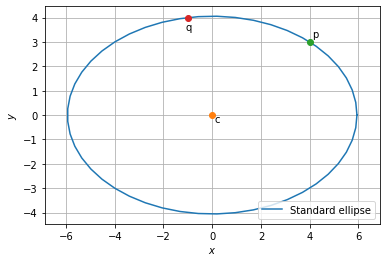
\includegraphics[width=\columnwidth]{figure5}
\caption{Standard Ellipse}
\label{fig:ellipse}	
\end{figure}

\eqref{eq:5}
can then be expressed as:
\begin{align}
\myvec{\vec{p}^T\vec{P}\\ \vec{q}^T\vec{Q}}\vec{d} &= \myvec{1\\1}\\
\myvec{16 & 9\\ 1 & 16}\vec{d} &= \myvec{1\\1}\label{eq:8}
\end{align}
Forming the augmented matrix and performing row reduction,
\begin{align}
\myvec{16 & 9 & 1\\ 1 & 16 & 1} 
\xleftrightarrow[R_2\leftarrow R_2-16R1,R_2\leftarrow-R_2]{R_2\leftrightarrow R1}
\myvec{1 & 16 & 1 \\ 0 & 247 & 15} 
\\
\xleftrightarrow[]{R_1\leftarrow 247R_1-16R_2}
\myvec{247 & 0 & 7 \\ 0 & 247 & 15} 
\\
\implies \vec{d} = \frac{1}{247}\myvec{7\\15}, \text{ or, } \vec{D} = \frac{1}{247}\myvec{7 & 0 \\ 0 & 15}
\end{align}
So, equation of ellipse is given by:
\begin{align}
\label{eq:12}
\vec{x}^T\myvec{7&0\\0&15}\vec{x}=247
\end{align}


The ellipse parameters center and axes are obtained from conics table in manual as
\begin{align}
\vec{c} = \vec{0};
\frac{1}{\sqrt{\lambda_1}}  = \sqrt{\frac{247}{7}},
\frac{1}{\sqrt{\lambda_2}}  = \sqrt{\frac{247}{15}}.
\end{align}
Clearly the \eqref{eq:12} satisfies all the constraints. So,it is one of the possible answers.
If standard ellipse is not considered then center $\vec{c}=\myvec{\beta\\0}$ can be taken anywhere on X axis in principle.The equation is given by:
\begin{align}
(\vec{x}-\vec{c})^T\vec{D}(\vec{x}-\vec{c})=1\label{eq:14}
\end{align}
$\because \vec{p}, \vec{q}$ satisfy \eqref{eq:14},
\begin{align}
\label{eq:ellipse_std_ab}
(\vec{p}-\vec{c})^T\vec{D}(\vec{p}-\vec{c}) &= 1,
\\
(\vec{q}-\vec{c})^T\vec{D}(\vec{q}-\vec{c}) &= 1,
\end{align}
which can then be written as:
\begin{align}
    2\times(\vec{p}^T\vec{D}-\vec{q}^T\vec{D})\vec{c}=\vec{p}^T\vec{D}\vec{p}-\vec{q}^T\vec{D}\vec{q}
\end{align}
Now $\vec{c}$ can be expressed as:
\begin{align}
2\vec{c}=(\vec{p}+\vec{q})+K\vec{D}^{-1}\vec{m}
\end{align}
Here K is any arbitrary constant and $\vec{m}$ satisfies ($\vec{p}^T-\vec{q}^T$)$\vec{m}=0$
Now,
\begin{align}
2\myvec{0&1}\vec{c}&=\myvec{0&1}(\vec{p}+\vec{q}+K\vec{D}^{-1}\vec{m})\\
0&=\myvec{0&1}(\vec{p}+\vec{q}+K\vec{D}^{-1}\vec{m})\label{eq:solve_1}
\end{align}
Similarly,
\begin{align}
2\myvec{1&0}\vec{c}&=\myvec{1&0}(\vec{p}+\vec{q}+K\vec{D}^{-1}\vec{m})\\
2\beta&=\myvec{1&0}(\vec{p}+\vec{q}+K\vec{D}^{-1}\vec{m})\label{eq:solve_2}
\end{align}
\eqref{eq:solve_1} and \eqref{eq:solve_2} can be written as:
\begin{align}
    \myvec{2\beta\\0}=\myvec{1&0\\0&1}(\vec{p}+\vec{q}+K\vec{D}^{-1}\vec{m})\\
    \myvec{2\beta\\0}=(\vec{p}+\vec{q}+K\vec{D}^{-1}\vec{m})
\end{align}
Using values $\vec{p}$,$\vec{q}$ and $\vec{D}$:
\begin{align}
   \myvec{2\beta\\0}=\myvec{3\\7}+T\myvec{\lambda_2 & 0 \\ 0 & \lambda_1}\myvec{1\\5}  
\end{align}
Here T=$\frac{K}{\lambda_1\lambda_2}$.Now,X axis is major axis so 
$\frac{\lambda_2}{\lambda_1}>1$
\begin{align}
    \frac{2\beta-3}{\frac{-7}{5}}>1\\
    \beta<0.8
\end{align}
Once we fix $\beta$,let
\begin{align}
\vec{p} = \myvec{4-\beta\\3} , \vec{q} = \myvec{– 1-\beta\\4}
\end{align}
Then $\vec{p}$,$\vec{q}$ will again satisfy \eqref{eq:2}.
Proceeding in a similar manner \eqref{eq:8} becomes:
\begin{align}
\myvec{(4-\beta)^2 & 9\\ (-1-\beta)^2 & 16}\vec{d} &= \myvec{1\\1}
\end{align}
The augmented matrix:
\begin{align}
    \myvec{(4-\beta)^2 & 9&1\\ (-1-\beta)^2 & 16&1}
\end{align}
RRE of augmented matrix:
\begin{align}
    \myvec{1&0&\frac{7}{7\beta^2-146\beta+247}\\0&1&\frac{5(3-2\beta)}{7\beta^2-146\beta+247}}
\end{align}
So,
\begin{align}
    \lambda_1=\frac{7}{7\beta^2-146\beta+247}\label{eq:18}\\
    \lambda_2=\frac{5(3-2\beta)}{7\beta^2-146\beta+247}\label{eq:19}\\
    \vec{D}=\myvec{\lambda_1&0\\0&\lambda_2}\label{eq:D}
\end{align}


\numberwithin{figure}{section}
\begin{figure}[!ht]
\centering
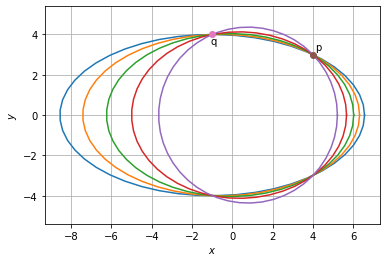
\includegraphics[width=\columnwidth]{figure5_1}
\caption{Ellipses passing through the two points with X axis as major axis}
\label{fig:ellipses}	
\end{figure}
\end{document}
